\subsection{Apache Jmeter}


Nach der offiziellen Dokumentation ist Apache Jmeter eine reine
Open-Source-Software, eine 100 \% reine Java-Anwendung, die von Stefano
Mazzocchi von der Apache Software Foundation entwickelt wurde, um das
Funktionsverhalten zu testen und die Leistung zu messen (vgl \cite{jmeter}). Jmeter kann
verwendet werden, um die Leistung von Webanwendungen oder einer Vielzahl
von Diensten zu analysieren und zu messen. Jmeter wurde ursprünglich zum
Testen von Webanwendungen oder FTP-Anwendungen verwendet. Heutzutage wird
es für funktionale Tests, Datenbankserver-Tests. Apache Jmeter kann
verwendet werden, um die Leistung statischer und dynamischer Ressourcen
sowie dynamischer Webanwendungen zu testen. Es kann verwendet werden, um
eine starke Belastung eines Servers, einer Gruppe von Servern, eines
Netzwerks oder eines Objekts zu simulieren, um dessen Stärke zu testen
oder um die Gesamtleistung unter verschiedenen Lasttypen zu analysieren.
Die wichtigsten Vorteile von Jmeter sind :

\begin{enumerate}

    \item \textbf{Open-Source-Lizenz}: Jmeter ist völlig kostenlos und erlaubt
     Entwicklern die Verwendung des Quellcodes für die Entwicklung.

    \item \textbf{Freundliche GUI}: Jmeter ist extrem einfach zu bedienen und es
    dauert nicht lange, sich damit vertraut zu machen.

    \item \textbf{Plattformunabhängig}: Jmeter ist eine 100\% reine
    Java-Desktop-Anwendung. Daher kann es auf mehreren Plattformen laufen.

    \item \textbf{Vollständiges Multithreading-Framework}: Jmeter ermöglicht die
    gleichzeitige und simultane Abtastung verschiedener Funktionen durch
    eine separate Thread-Gruppe.

    \item \textbf{Visualisierung des Testergebnisses}: Das Testergebnis kann in
    verschiedenen Formaten wie Diagramm, Tabelle, Baum und Protokolldatei
    angezeigt werden.

    \item \textbf{Skalierbarkeit}: Jmeter  unterstützt auch Visualisierungs-Plugins,
    mit denen Tests erweitert werden können.

    \item \textbf{Mehrere Teststrategien}: Jmeter unterstützt viele
    Teststrategien wie Lasttests, verteilte Tests und funktionale Tests.

    \item \textbf{Simulation}: Jmeter kann mehrere Benutzer mit gleichzeitigen Threads
    simulieren und eine hohe Last auf die zu testende Webanwendung erzeugen.

    \item \textbf{Unterstützung mehrerer Protokolle}: Jmeter unterstützt nicht
    nur das Testen von Webanwendungen, sondern bewertet auch die
    Leistung von Datenbankservern. Alle Basisprotokolle wie HTTP, JDBC,
    LDAP, SOAP, JMS und FTP werden von Jmeter unterstützt.

    \item \textbf{Aufzeichnung und Wiedergabe}: Jmeter ermöglicht das Aufeichnen
    von Benutzeraktivität im Browser und hilft dabei sie in einer
    Webanwendung zu simulieren.

    \item \textbf{Skript-Test}: Jmeter kann mit Bean Shell für automatisierte Tests
    integriert werden.

\end{enumerate}

Im Allgemeinen hat Jmeter ein vereinfachtes Funktionsprinzip. Es simuliert
eine Gruppe von Benutzern, die Anfragen an einen Zielserver senden, und
gibt Statistiken zurück, die die Leistung/Funktionalität des Zielservers/der
Zielanwendung in Tabellen und Diagrammen zeigen (siehe \Cref{fig:jmeter-prinzip}).

\begin{figure}[H]
    \centering
    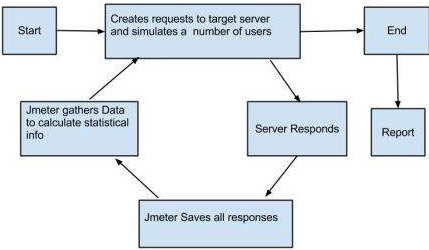
\includegraphics[scale=0.5]{images/jmeter-princip}
    \caption{Funktionsweise von Jmeter} \label{fig:jmeter-prinzip}
\end{figure}

Jmeter wird normalerweise  über seine grafische Benutzeroberfläche
bedient. Es ist  jedoch möglich, Tests mit der grafischen
Benutzeroberfläche zu erstellen und sie in einem Docker-Container auf einer
Anwendung auszuführen. Dieses  Prinzip wurde zum Testen der beiden Versionen
von jExam verwendet und wird  im nächsten Abschnitt vorgestellt.






